{
	\color{solution}
	\begin{enumerate}
		\item \underline{INTERPOLATION:}
		\begin{itemize}
			\item 
			Aim: We want to find $c_0,c_1,c_2$, such that\\
			$f(z_1)=c_0\cdot 1+c_1\cdot z_1+c_2\cdot z_1^2 = y_1$,\\
			$f(z_1)=c_0\cdot 1+c_1\cdot z_2+c_2\cdot z_2^2 = y_2$,\\
			$f(z_1)=c_0\cdot 1+c_1\cdot z_3+c_2\cdot z_3^2 = y_3$.
			\item 
			With $A = (a_{ij})_{ij} := (z_i^{j-1})_{ij},~ x:= (c_0,c_1,c_2)^T,~b:= (y_1,y_2,y_3)^T$ this is equivalent to:
			$$
			Ax = b.
			$$
			\item 
			Inserting the data points $(z_i,y_i)$ gives: 
			\begin{align*} 
			A = \begin{array}{r}
			\textcolor{violet}{\text{(I)}}\\
			\textcolor{violet}{\text{(II)}}\\
			\textcolor{violet}{\text{(III)}}
			\end{array}
			\begin{pmatrix} 
			1&-1&1\\
			1&0&0\\
			1&1&1\end{pmatrix}, ~~
			b =\begin{pmatrix} -1\\3\\1\end{pmatrix}.
			\end{align*}
			$\textcolor{violet}{\text{(II)}}\Rightarrow x_1 = 3$\\
			$\textcolor{violet}{\text{(I)}}\Rightarrow \underbrace{x_1}_{\textcolor{blue}{=3}}-x_2+x_3=-1 \ \ \Leftrightarrow\ \ x_3=x_2-4$\\
			$\textcolor{violet}{\text{(III)}}\Rightarrow \underbrace{x_1}_{\textcolor{blue}{=3}}+x_2+\underbrace{x_3}_{\textcolor{blue}{=x_2-4}} = 1\ \ \Leftrightarrow\ \ x_2 = 1$
			\item 
			All in all: $$x=\begin{pmatrix} c_0\\c_1\\c_2\end{pmatrix}
			=\begin{pmatrix}3\\1\\-3\end{pmatrix}.$$
			\item 
			Thus, our fitting parabola is given by:
			$$
			\textcolor{blue}{f(z)=3+z-3z^2}.
			$$
			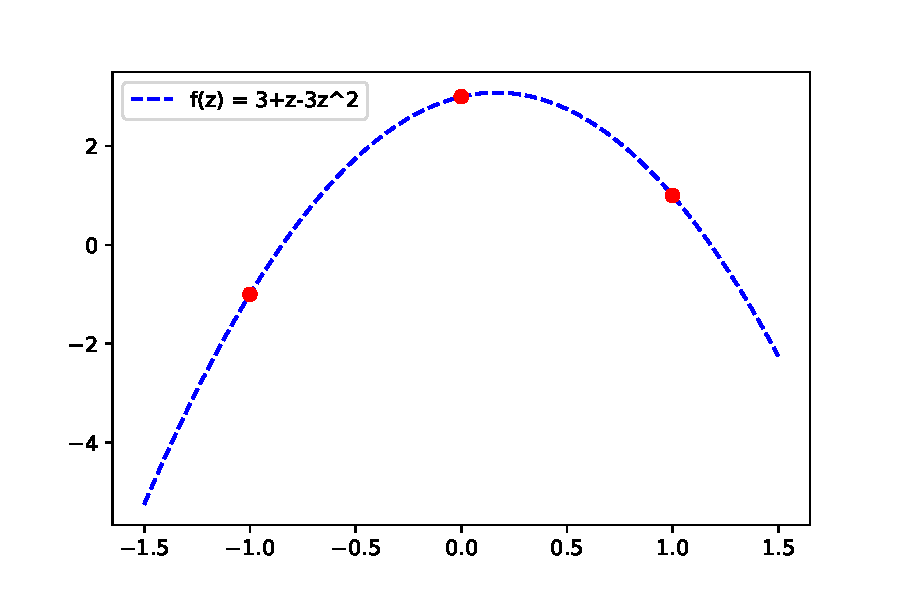
\includegraphics[width=0.5\textwidth]{interpolation.pdf}
		\end{itemize}
		\item \underline{LINEAR REGRESSION:}
		\begin{itemize}
			\item 
			Aim: Find $c_0,c_1$ such that
			$$
			f(z_i) = c_0+c_1z_i\approx y_i~~ \forall i=1,2,3.
			$$
			\item 
			As above we define
			\begin{align*}
			&A :=(a_{ij})_{ij}=(z_i^{j-1})_{ij}
			=\begin{pmatrix}1&z_1\\1&z_2\\1&z_3\end{pmatrix}
			=\begin{pmatrix}1&-1\\1&0\\1&1\end{pmatrix},\\
			&x:=\begin{pmatrix}c_0\\c_1\end{pmatrix},~~ b:=\begin{pmatrix}y_1\\y_2\\y_3\end{pmatrix}.
			\end{align*}
			\item Then by construction of $A, x$ and $b$ we find:
			$$
			\|{Ax-b}\|_2^2 = {\Bigg\Vert \underbrace{\begin{pmatrix}1&z_1\\1&z_2\\1&z_3\end{pmatrix}\begin{pmatrix}c_0\\c_1\end{pmatrix}}_{\textcolor{blue}{=\begin{pmatrix}c_0+z_1c_1\\c_0+z_2c_1\\c_0+z_3c_1\end{pmatrix}=\begin{pmatrix}f(z_1)\\f(z_2)\\f(z_3)\end{pmatrix}}}-\begin{pmatrix}y_1\\y_2\\y_3\end{pmatrix}}\Bigg\Vert_2^2=\\
			\Bigg\lVert{\begin{pmatrix}f(z_1)-y_1\\f(z_2)-y_2\\f(z_3)-y_3\end{pmatrix}}\\
			\Bigg\rVert_2^2\stackrel{\textcolor{blue}{\text{Def. of}\ \|{\cdot}\|_2}}{=}\sum_{i=1}^{3}(f(z_i)-y_i)^2.
			$$
			\item 
			We now solve the $\textcolor{red}{\text{normal equation}}$ $$A^TAx = A^Tb$$
			to determine the solution of the least squares problem:
			$$
			\min_{x=(c_0,c_1)\in\mathbb{R}^2} \|{Ax-b}\|_2^2 = \min_{c_0,c_1}\sum_{i=1}^{3}[(c_0+c_1z_i)-y_i]^2.
			$$
			\item 
			We find
			\begin{align*} 
			&A^TA = \begin{pmatrix}1&1&1\\-1&0&1\end{pmatrix}
			\begin{pmatrix}1&-1\\1&0\\1&1\end{pmatrix} =\begin{pmatrix}3&0\\0&2\end{pmatrix},\\
			&A^Tb =\begin{pmatrix}1&1&1\\-1&0&1\end{pmatrix}\begin{pmatrix}-1\\3\\1\end{pmatrix}=\begin{pmatrix}3\\2\end{pmatrix}.
			\end{align*}
			\item 
			Thus:
			$$
			A^TAx = A^Tb~~\Leftrightarrow~~ \begin{pmatrix}3&0\\0&2\end{pmatrix}
			\begin{pmatrix}c_0\\c_1\end{pmatrix}
			=\begin{pmatrix}3\\2\end{pmatrix}~~ \Leftrightarrow~~ \begin{matrix}c_0=1\\c_1=1\end{matrix}.$$
			\item 
			Therefore the best linear fit in the least squares sense is given by
			$$
			\textcolor{violet}{g(z) = 1+z}.
			$$
			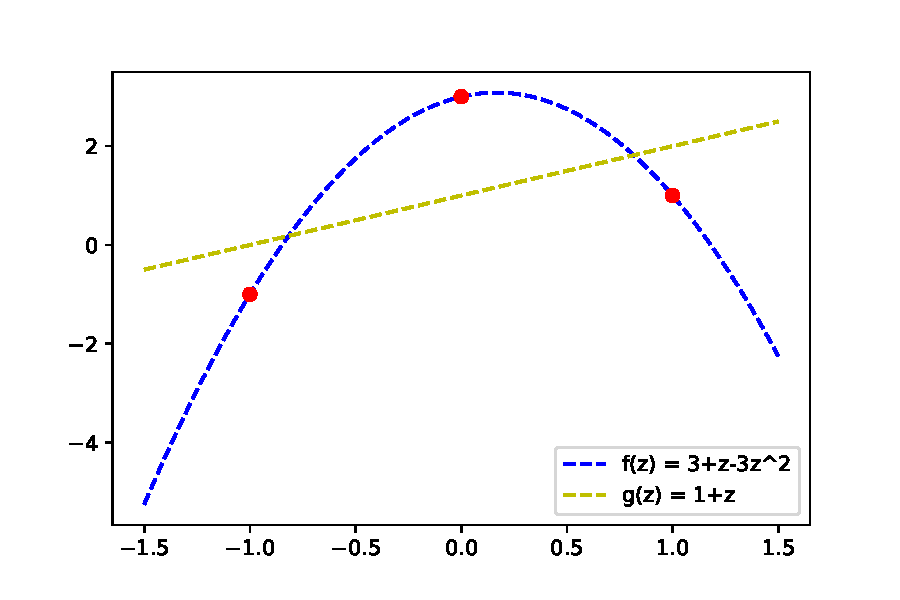
\includegraphics[width=0.5\textwidth]{regression.pdf}
		\end{itemize}
	\end{enumerate}
}